\documentclass{beamer}
\mode<presentation>
{
  \usetheme{AnnArbor}      % or try Darmstadt, Madrid, Warsaw, ...
  \usecolortheme{beaver} % or try albatross, beaver, crane, ...
  \usefonttheme{default}  % or try serif, structurebold, ...
  \setbeamertemplate{navigation symbols}{}
  \setbeamertemplate{caption}[numbered]
} 

\usepackage[english]{babel}
\usepackage[utf8x]{inputenc}
\usepackage{graphicx}

\title[Understandin regression results]{Regression Vs. ANOVA:\\Is a main effect really a main effect?}
\author[A. Capelier-Mourguy]{Arthur Capelier-Mourguy}
\institute{Lancaster University}
\date{17th of July 2018}

\begin{document}

\begin{frame}
  \titlepage
\end{frame}

\begin{frame}{Outline}
  \tableofcontents
\end{frame}

\section{Introduction}

\subsection{Defining the problem}

\begin{frame}{Defining the problem}

  \begin{exampleblock}{What you might see}
  We defined a regression model $\texttt{Score} \sim \texttt{\alt<1>{Condition*PrePost}{Condition + PrePost + Condition:PrePost}}$.\pause
  
  \pause
  We found a significant main effect of Condition, with higher scores in the group A than in the group B.
  
  \pause
  $[$Table with parameter estimates and statistics$]$
  \end{exampleblock}
  \vspace{1em}
  \pause
  \begin{itemize}
    \item What does the regression model actually do?
    \item What do the parameter values in the table mean?
    \item What does ``main effect'' mean in the context of a regression?
  \end{itemize}
  \vspace{1em}
  \pause
  \centering{\emph{All stats in R have the same syntax}}

\end{frame}

\subsection{Content of this talk}

\begin{frame}{What too expect from this talk?}

  \vfill
  \begin{block}{What this talk is about}
    \begin{itemize}
      \item Demonstrate how ANOVA and regression results differ
      \item Detail what parameters in a regression model mean and do
    \end{itemize}
  \end{block}
  \vfill
  \pause
  \begin{block}{What this talk is not about}
    \begin{itemize}
      \item How to use R
      \item How to build a good mixed-effects model
      \item The $p$-value debate
    \end{itemize}
  \end{block}
  \vfill

\end{frame}

\section{Toy Example}

\subsection{Using categorical variables only}

\begin{frame}{The simulated data}
  
  \vfill
  Assessing stress levels after and before a 30 minutes intervention, ``mindfulness meditation'' or ``video games''.
  \vfill
  \pause
  \begin{center}
  \begin{overlayarea}{4in}{2in}
  \only<2>{\centering{\includegraphics{../src/CategoricalBarplot.pdf}}}
  \only<3>{\centering{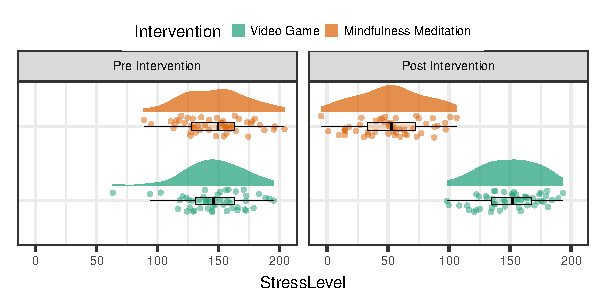
\includegraphics{../src/CategoricalRaincloud.pdf}}}
  \end{overlayarea}
  \end{center}
  \vfill

\end{frame}

\begin{frame}{Regression and ANOVA results}

\end{frame}

\begin{frame}{Graphically understanding the regression results}

\end{frame}

\subsection{Using continuous variables}

\begin{frame}{Changes to the simulated data}

\end{frame}

\begin{frame}{Regression results}

\end{frame}

\begin{frame}{Graphically understanding the regression results}

\end{frame}

\section{Real Data Example}

\subsection{Methods}

\begin{frame}{The experiment in a nutshell}

\end{frame}

\subsection{Results}

\begin{frame}{Impact of the choice of reference levels}

\end{frame}

\section{Conclusion}

\begin{frame}{What's the take home message?}

\end{frame}

\end{document}
